% This is LLNCS.DEM the demonstration file of
% the LaTeX macro package from Springer-Verlag
% for Lecture Notes in Computer Science,
% version 2.4 for LaTeX2e as of 16. April 2010
%
\documentclass{llncs}
%
\usepackage{makeidx}  % allows for indexgeneration
\usepackage[utf8]{inputenc}
\usepackage{graphicx}
\usepackage{float}
\usepackage{placeins}
%
\begin{document}
\tableofcontents
%
%\mainmatter              % start of the contributions
%
\title{Solving an optimization problem employing restraint programming}
%
\titlerunning{Restraint Programming}  % abbreviated title (for running head)
%                                     also used for the TOC unless
%                                     \toctitle is used
%
\author{João Cabral\inst{1} \and João Mota\inst{2}}
%
\authorrunning{João Cabral \and João Mota} % abbreviated author list (for running head)
%
%%%% list of authors for the TOC (use if author list has to be modified)
\tocauthor{João Cabral, João Mota}
%
\institute{Faculdade de Engenharia da Universidade do Porto, Porto, Rua Roberto Frias s/n 4200-465, Portugal,\\
\email{(up201303462, up201304395)@fe.up.pt}}

\maketitle              % typeset the title of the contribution

\begin{abstract}
This paper goes over the theoretical and practical aspects of the resolution of an optimization problem,
namely the synthesis of a schedule for a language school, employing restraint programming, more precisely, 
SICSTUS Prolog's restraint programming capabilities.
The paper contains a description of the problem, a detailed analysis of the aproach used to solve it, 
an explanation of how the solution should be interpreted, a description of obtained results and, finally, conclusions.
%n ta bem isto...

\keywords{optimization, restraint programming, PROLOG}
\end{abstract}
%
%ISTO TA A FICAR APERTADO D PAGS, SE EXCEDER TIRA-SE OS VERBATIMS TODOS E OS PROFS PODEM IR LER AOS ANEXOS Q SE FODEM
\section{Introduction}
Within the context of the Logic Programming course of MIEIC, the authors of this paper were asked to solve an optimization problem in the most efficient way possible using the restraint programming capabilities of SICStus PROLOG. The optimization problem under study is that of producing a working schedule for a language school that maximizes it's (monetary) gains,  given a number of inputs of variable length, aswell as a number of restrictions of various types. The rest of the paper is structured as follows:

\begin{itemize}
	\item Problem Description - A detailed description of the problem that's under study in this paper.
	\item Approach - The authors' approach to the modelization of the problem as a Constraint Satisfaction Problem (henceforth called CSP)
	\item Solution Presentation - Explanation of the predicades that allow a user to interpret the output of the implemented solution.
	\item Results - Examples of different instances of the problem with differing complexities, aswell as a discussion of the temporal and spatial efficiency of the implemented solution.
	\item Conclusions and Future Work - Discussion of the conclusions to withdraw from the obtained results.
	\item References - Any and all work the authors' used to further the completion of the proposed task.
	\item Annex - Source code, Results, Data files regarding the program's efficiency
\end{itemize}

\section{Problem Description}
As was mentioned in the introduction, the optimization problem under study in this paper is that of producing a working schedule for a language school that maximizes it's gains, given a number of inputs of varialbe length, coupled with a number of restricitons.  The inputs consist of a list of teachers, a list of registrations for the language courses, a list of language courses provided and the number of rooms available at the hypothetical school. As for restrictions, they are as follows:

\begin{itemize}
	\item A student will pay an hourly amount for the attendance of a course, which will differ based on the course.
	\item A teacher can work at most 15 hours per week, and will only work on specific days
	\item A teacher will earn a certain amount per hour, based on the language taught. If the teacher is working more than 10 hours per week, the earnings for the excess will be decreased by 20\%.
	\item Each language course, if taught, will have no less than 2 weekly hours, and no more than 4.
	\item Each course can be frequented by at most 15 students
	\item The school has a finite number of classrooms
\end{itemize}

There are, of course, other, implicit, restrictions, such as the fact that a teacher cannot teach a language course for a language that he's not qualified to teach, or the fact that a course cannot be taught if there are no students registered for it, or if there's no qualified teachers to teach it.

\section{Approach}
In this section, the more technical aspects of solving the problem are discussed, such as the modelization of the problem as a CSP and the implementation of its restrictions. It also goes over the search strategies employed in the program's labeling phase.

\subsection{Problem Modelization}
In order to function, the program implemented by the paper's authors to solve the problem unser study needs to be fed a number of inputs. As was mentioned before, these consist of a list of teachers, a list of course registrations, the list of available courses and the number of available rooms. The list of teachers is implemented as follows:
\begin{verbatim}
	[[TeacherIndex, [LanguageIndex-PayPerHour|OtherLanguages], [DayAvailable|OtherDays] ]
	| OtherTeachers]
\end{verbatim}

Where the first list within a teacher represents the languages that teacher's qualified to teach (and it's hourly pay) and the second represents the indexes of the days a teacher's available to teach.

The course registrations are implemented as follows:
\begin{verbatim}
	[LanguageIndex-NumberOfRegistrations|OtherLanguages]
\end{verbatim}

The available courses list is implemented as follows: 
\begin{verbatim}
	[LanguageIndex-HourlyCost|OtherLanguages]
\end{verbatim}

The number of rooms in this problem is interpreted by the paper's authors as the number of classes that can be taught simultaneously each day. This is done for the sake of simplifying the problem, otherwise the solution would have to take into account the concept of hours and different classes for the same course.

Given all of these inputs, the program will produce a solution that's formatted as follows:
\begin{verbatim}
	[LanguageIndex-[[DayIndex, HoursTaught, TeacherIndex|OtherDays]]|OtherLanguages]
\end{verbatim}

Where the list attached to every LanguageIndex consists of a listing of the hours of class taught each day of the week, and the teacher that's assigned to teach them.

\subsection{Decision Variables}
As was mentioned in the section above, the solution is formatted as follows:
\begin{verbatim}
	[LanguageIndex-[[DayIndex, HoursTaught, TeacherIndex|OtherDays]]|OtherLanguages]
\end{verbatim}

In the problem under study, the decision variables are HoursTaught and TeacherIndex, LanguageIndex and DayIndex being fixed in order to be able to present the solution in a coherent, comprehensive way.

The domain for HoursTaught is 0-4, seeing as the most hours of class a course can have per week is 4. The domain for TeacherIndex, however, is rather complex. It'll be the list of  TeacherIndexes with hours to spare (from the weekly 15 they are alloted), who are qualified to teach the language in question and are not teaching any other language that day (this is due to the way the concept of classrooms is interpreted in the context of this solution, which is explained in the section above this one). In the particular case of courses that didn't open for lack of students or teachers, the TeacherIndex variable will assume the value -1.

\subsection{Constraints}
% FALTA BOTAR AQUI CENAS
The constraints for this particular problem are listed in section 2. As such this section will focus mainly on constraints' implementation aspects. All constraints concerning monetary values are approached during the profit calculating phase of the solution, which is further explained in the next section of this paper. For the constraint concerning the number of hours of class a certain course can have per week, the program will gather the values for the hours taught each day and say that their sum must be grater than or equal to 2 and lesser than or equal to 4. 

\begin{verbatim}
restrict_course_times([]).
	restrict_course_times([_-[[_,H1,_],[_,H2,_],[_,H3,_],[_,H4,_],[_,H5,_]]|T]):-
		sum([H1,H2,H3,H4,H5],#=<,4),
		sum([H1,H2,H3,H4,H5],#>=,2),
		restrict_course_times(T).
\end{verbatim}

There are, however, exceptions to this restriction in the authors' implementation of a solution, where a course can have 0 weekly hours taught when it doesn't have anyone to attend or teach it (effectively signifying that this course didn't open).

Concerning the restriction that a teacher can teach at most 15 hours per week, a number of predicates are in place that process and convert the input into formats that make it easy to gather the variables that concern the number of hours a teacher teaches per week. It is then said that the sum of these variables cannot exceed 15 (the code concerning this can be viewed in the annex, and will not be replicated here for reasons of spatial economy).

In the interest of reducing the domain and the search space to feasible levels the authors implemented a further constraint that limits each class to only having a 2 hour duration. This means that each course can have either one 2 hour class or 2 2 hour classes.

\subsection{Evaluation Function}
Since the program has the goal of maximizing the monetary gains for the school, the evaluation function for the problem at hand is the total weekly gains of the school. The value for the total weekly gains of the school is calculated by summing the daily gains for each language, which can be calculated using the following formula:

\begin{equation}
	profit = hoursTaught*((students*pricePerHour)+(-teacherSalary))
\end{equation}

The predicates below are used to calculate the profit:
%ATUALIZAR AQUI SE ISTO FOR MUDADO
\begin{verbatim}
make_profit([], _, _, _,_, 0).
make_profit([Solucao|Solucoes], Linguas, Professores,TabelaCustos, Candidaturas, Lucro):-
	make_profit_language(Solucao, Linguas, Professores, TabelaCustos, Candidaturas, LucroLingua),
	make_profit(Solucoes, Linguas, Professores, TabelaCustos, Candidaturas, LucroResto),
	Lucro #= LucroResto+LucroLingua.

make_profit_language(Lingua, Linguas, Professores, TabelaCustos, 
Candidaturas, LucroLingua):-
	Lingua = IndiceL-Dias,
	make_profit_day(Dias, Linguas, Professores, TabelaCustos, 
	Candidaturas, IndiceL, LucroLingua).
make_profit_day([], _, _,_, _, _, 0).
make_profit_day([Dia|OutrosDias], Linguas, Professores, TabelaCustos,
 Candidaturas, IndiceL, LucroDia):-
	Dia = [_, Horas, Professor],
	table([[Professor, IndiceL, Remuneracao]],TabelaCustos),
	Prejuizo #= Remuneracao * Horas,
	member(IndiceL-Preco, Linguas),
	member(IndiceL-NumeroCandidatos, Candidaturas),

	Lucro #= Preco*NumeroCandidatos*Horas,
	LucroDiaAtual #= (Lucro-Prejuizo),
	make_profit_day(OutrosDias, Linguas, Professores,TabelaCustos, 
	Candidaturas, IndiceL, LucroRest),
	LucroDia #= LucroRest + LucroDiaAtual.
\end{verbatim}

Then, in the labeling phase, the program is told to maximize Profit, as seen here:

\begin{verbatim}
labeling([ff,leftmost,down,maximize(Profit)], Flat).
\end{verbatim}

\subsection{Search Strategy}
Establishing an optimal search strategy for this problem presents difficulties due to the large variety of valid inputs possibly benefitting from a variety of different options. The search strategies selected are presented with a brief rationale for their choice. The tests run on each set of options are show on table \ref{table:speedup}. 


For choice making the \textit{step} option was selected over the common \textit{bisect} option. It allows for a speedier pruning of the domain space because, in conjunction with the \textit{down} option it leads to higher profit solutions as the first solutions. The discovery of high profit solutions early in the branch-and-bound algorithm allows for larger prunings to be made on the search tree. This results in marginally faster times when compared to \textit{bisect}.

Given the goals of maximizing the cost being closely tied with maximizing the number of hours taught at the school the obvious choice of searching though domains in descendant order with the option \textit{down} was made. This resulted in significant speedups when compared to the default option \textit{up}.


\begin{table}[]
\caption{6 professors, 5 languages, 4 classrooms test}
\label{table:speedup}
\centering
\begin{tabular}{l|l|l|}
\cline{2-3}
                                      & time(s) & speedup \\ \hline
\multicolumn{1}{|l|}{up,bisect,ff}    & 520.052 & 1x      \\ \hline
\multicolumn{1}{|l|}{down,bisect,ff,} & 20.725  & 25.09x  \\ \hline
\multicolumn{1}{|l|}{down,step,ff}  & 21.349  & 25.55x  \\ \hline
\end{tabular}

\end{table}
 
 \section{Solution Presentation}
 After the labeling phase, the solution is presented in a way that isn't easily legible by users who have no knowledge of the program's implementation. To aid in the observation and interpretation of the solution, the authors created a predicate which converts it to a more understandable format.  Here's an example of a possible solution:
 
 \begin{verbatim}
 Language 0 Time Table
 _______________
Language 1 Time Table
_______________
Language 2 Time Table
_______________
Language 3 Time Table
_______________
Monday - 2 hours with professor 0
Tuesday - 2 hours with professor 0

Language 4 Time Table
_______________
Wednesday - 2 hours with professor 4
Friday - 2 hours with professor 0

Language 5 Time Table
_______________
Thursday - 2 hours with professor 3

O lucro total obtido e de 994
Resumptions: 967755
Entailments: 124262
Prunings: 348556
Backtracks: 1566
Constraints created: 749
O resultado foi obtido em 0.140 segundos.
 \end{verbatim}
 
 As can be seen above, a time table is created for each language in which only the days in which the class is taught are displayed, along with the number of hours taught that day and the teacher who teaches them. This is achieved via the creation of 5 predictes that make the connection between the index of days and the actual day, coupled with predicates that format and write the information on the screen. (This code that does this can be viewed in the annex, namely in the predicate printSolution).
 
 \section{Results}
The following graphics plot the performance results obtained with the modeling and constraints chosen, when increasing the number of classrooms, professors and languages being taught. All other variables are not changing in each series, to provide a accurate representation of the performance of the program.

\begin{figure}[h]
  \centering
    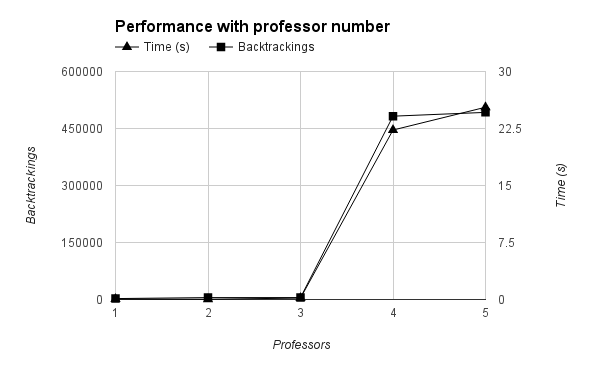
\includegraphics[width=1\textwidth]{professor.png}
\end{figure}


\begin{figure}[h]
  \centering
    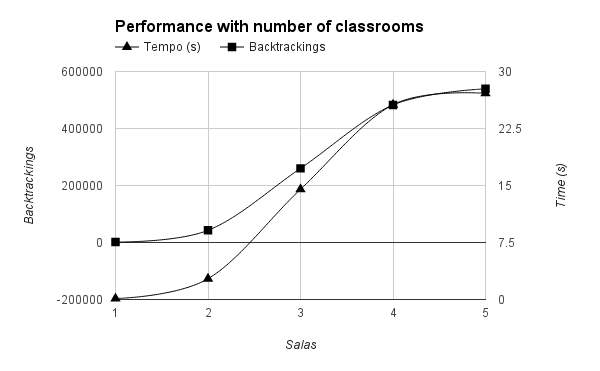
\includegraphics[width=1\textwidth]{classrooms.png}
\end{figure}


\begin{figure}[h]
  \centering
    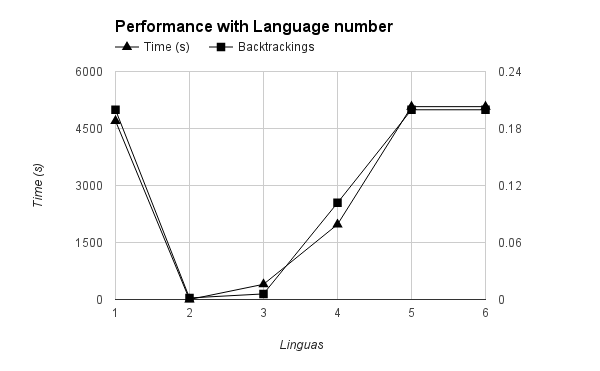
\includegraphics[width=1\textwidth]{language.png}
\end{figure}
 
\FloatBarrier
 \section{Conclusions and Future Work}
 Having implemented a solution to the problem under study, the paper's authors are able to appreciate the advantages of employing restraint programming in the solving of problems that are similar to the one studied here. Indeed, the implemented solution shows that the use of this technology allows for a relatively simple implementation of a solution, when compared to possible implementations using other technologies.

It is possible to observe the effect on performance of the establishment of constraints, which works somewhat conterintuitively in that the imposition of further constraints can be extremely beneficial for performance, achieving sometimes surprising speedups by imposing constraints. One should however note that some constraints, particularly those that are not global, can also significantly degrade performance. The use of reification in particular, which the authors attempted in one of the first implementations, proved to be too costly despite the advantages in code simplicity it provided. It was thus replaced with a global constraint.  

The solution now presented suffers from a significant degradation in performance as the problem size expands. This is partly due to the intrinsic characteristics of the problem that mandates the use of multiple decision variables with  relatively large domains, compounded by the fact that each decision made by the solver can have a relatively modest effect on the size of the remaining domains when it propagates. However, the modelization chosen is also not optimal as it allows, within the constraints of the problem, for multiple, equivalent, solutions that while valid and distinct do not represent any sort of improvement or even to relevant alternatives. For example, professors who can give classes in a large range of days can provoke an exponential growth of the solution space, even when constrained to the optimal solutions, which the solver is forced to explore. Relevant future work includes improvements to the modelization of the problem and possibly the implementation of a heuristic of selection of domain variables to allow for quicker constraint of the domains and possibly discarding exploration of useless, equivalent paths in the search tree.
%aspetos a melhorar???
 
%
% ---- Bibliography ----
%
\begin{thebibliography}{5}
%
\bibitem {clar:eke}
Clarke, F., Ekeland, I.:
Nonlinear oscillations and
boundary-value problems for Hamiltonian systems.
Arch. Rat. Mech. Anal. 78, 315--333 (1982)

\bibitem {clar:eke:2}
Clarke, F., Ekeland, I.:
Solutions p\'{e}riodiques, du
p\'{e}riode donn\'{e}e, des \'{e}quations hamiltoniennes.
Note CRAS Paris 287, 1013--1015 (1978)

\bibitem {mich:tar}
Michalek, R., Tarantello, G.:
Subharmonic solutions with prescribed minimal
period for nonautonomous Hamiltonian systems.
J. Diff. Eq. 72, 28--55 (1988)

\bibitem {tar}
Tarantello, G.:
Subharmonic solutions for Hamiltonian
systems via a $\bbbz_{p}$ pseudoindex theory.
Annali di Matematica Pura (to appear)

\bibitem {rab}
Rabinowitz, P.:
On subharmonic solutions of a Hamiltonian system.
Comm. Pure Appl. Math. 33, 609--633 (1980)

\end{thebibliography}


\end{document}
